\documentclass[letterpaper,11.5pt]{scrartcl}
\usepackage{totcount}
% \documentclass[11pt]{report}
% \documentclass{report}
% \documentclass{book}
\usepackage[bookmarks, hidelinks]{hyperref}
\usepackage{amssymb,amsmath}
\usepackage[title]{appendix}
% \usepackage{fullpage}
\usepackage{tabulary}
\usepackage{tabularx}
\usepackage{float}
% \usepackage[margin=0.50in]{geometry}
\usepackage[margin=1.00in]{geometry}

\usepackage{booktabs}
\usepackage{pslatex}
\usepackage{apacite}
\usepackage{caption}
% \usepackage{subcaption}
\usepackage{wrapfig}
\usepackage[english]{babel}
\usepackage{lmodern}
\usepackage{setspace}
\doublespace
% \usepackage{url}
\usepackage{bigfoot}
\usepackage[export]{adjustbox}
\setlength\intextsep{0pt}

% Colored comments 
\usepackage{color}
\definecolor{myorange}{RGB}{240, 96, 0}
\newcommand{\mt}[1]{{\textcolor{myorange} {({\tiny MT:} #1)}}}

\definecolor{myblue}{RGB}{30,144,255}
\newcommand{\jhj}[1]{{\textcolor{myblue} {({\tiny JHJ:} #1)}}}

\definecolor{mypurple}{RGB}{148,0,211}
\newcommand{\cm}[1]{{\textcolor{mypurple} {({\tiny CM:} #1)}}}

\definecolor{mygreen}{RGB}{26, 153, 51}
\newcommand{\ps}[1]{{\textcolor{mygreen} {({\tiny PS:} #1)}}}

\newtotcounter{citnum} %From the package documentation
\def\oldbibitem{} \let\oldbibitem=\bibitem
\def\bibitem{\stepcounter{citnum}\oldbibitem}

\usepackage{graphicx}

\title{Uncertainty in social learning evolution}

\author{{}}

\begin{document}
\maketitle

\newcommand{\pisub}[1]{\pi_{\mathrm{#1}}}
\newcommand{\pilow}{\pisub{low}}
\newcommand{\pihigh}{\pisub{high}}
\newcommand{\piI}{\langle \pisub{I} \rangle}
\newcommand{\piS}{\langle \pisub{S} \rangle}
\newcommand{\ledger}{\bar\pi_{ib}}

\newcommand{\meanvar}[1]{\langle #1 \rangle}
\newcommand{\meansl}{\meanvar{s}}
\newcommand{\meanpi}{\meanvar{\pi}}
\newcommand{\meansoc}{\meanvar{\pi_\mathrm{S}}}
\newcommand{\meanasoc}{\meanvar{\pi_\mathrm{A}}}
\newcommand{\meanT}{\meanvar{T}}

\newcommand{\bandit}{\text{Bandit}_b(0, 1)}

\begin{abstract}

Social learning is essential to survival. It is likely to evolve when it is more
efficient than asocial, trial-and-error learning. Theoretically, some uncertainty is
necessary for social learning to be necessary, but too much uncertainty makes
social information useless. This fact is empirically
supported across biology and human sciences. However, we lack a theoretical
framework to predict the effects of specific classes and types of uncertainty on social
learning evolution. Furthermore, existing models and experimental operationalizations of
uncertainty are ambiguously related, and 
tend to only consider a small number of sources of uncertainty and behavioral
choices.  Here we use evolutionary agent-based modeling to consolidate
models of uncertainty in social learning evolution to improve on these
shortcomings. We model a time-varying environment with a varying number
of possible behaviors agents could perform to acquire payoffs.
We show that environmental variability, ambiguous payoffs, 
larger decision sets, and shorter agent lifespans interact to 
affect social learning evolution in complex ways that 
sometimes caused evolution to be highly uncertain about whether social learning was
the optimal strategy. 
Our work strengthens social evolution theory that could help 
guide human, non-human, and artificial intelligence towards optimal responses 
to existential threats and new opportunities.\footnote{This document contains
\total{citnum} references.}  
\end{abstract}

\section{Introduction}

Social learning is essential to human and other species' everyday life and survival.
It allows individuals to solve problems when acquiring information from others is
more efficient than learning on one's own~\cite{Laland2004}. Theory predicts that
social learning should be favored in contexts with greater
uncertainty~\cite{BoydRicherson1985,Henrich1998}, up to a
point~\cite{Rogers1988,Feldman1996}; this prediction has received some empirical
support across species~\cite{McElreath2005,Kendal2018,Allen2019}.  However, the
meaning of the term \emph{uncertainty} often conflates environmental variability,
spatial heterogeneity, ambiguity or uncertainty about payoff structure, and other
variability that could be plausibly interpreted as \emph{uncertainty}.  Many models
of social learning evolution do not account for 
individual-level cognition~\cite{Heyes2016}, though humans
clearly have evolved cognitive mechanisms for dealing with 
uncertainty generally~\cite{Gershman2019,Schulz2019}.
Furthermore, social learning evolution theory tends to be organized around an
increasing number of modeling choices~\cite[Figure 1]{Kendal2018} instead
of around broader contextual assumptions such as uncertainty conditions. It remains
an outstanding question, then, to identify how different contexts and forms of
uncertainty might combine to affect social learning evolution in complex ways.
Answering this question is critical for understanding human behavior adapting to a
rapidly changing world, both to mitigate existential
threats~\cite{Moya2020,Jones2021}, and to captialize on new opportunities such as
transitioning to clean energy use and
production~\cite{NatureEnergyEditorialPromisesPremises2018,Brisbois2022}.
We will answer this question about how uncertainty drives evolution, including
identifying regimes where evolution itself is highly uncertain and often 
leads populations into suboptimal learning strategies~\cite{Rogers1988}.

\mt{This paragraph is a first try to introduce the four uncertainty dimensions
with examples to illustrate the problem we are answering.
I outlined the next paragraph to get into more details of social learning:
how cultural evolution works; conformity, success-biased, etc. Cristina, please
edit this.} 
To gain a more systematic understanding of uncertainty and social learning
evoluiton, we identified four common classes of ecological
uncertainty (``principal components'' of uncertainty) used as factors
in social learning evolution models: (1) environmental variability; (2) payoff
ambiguity (difference between best behavior choice and others); (3) 
selection set size (number of ecologically possible behaviors); and 
(4) the lifespan of agents. These were chosen because modeling and empirical 
study designs across taxa tend use one or more of these uncertainty dimensions.
Environmental variability is sometimes modeled as catastrophic and 
happens only once in an individual's lifetime~\cite{Rogers1988}, or may be
modeled as occurring with a fixed or variable
probability~\cite{Feldman1996,McElreath2005}---in these examples environments
can only be in one of two states. Payoff ambiguity is sometimes in the form
of differences in expected payoffs arising from different
behaviors or strategies~\cite{Enquist2007,Rendell2010}
or by varying the standard deviation of payoffs~\cite{McElreath2005}. 
Selection set size is often limited to one size throughout social learning
evolution studies: empirical studies of \emph{bombus terresteris} (bumble
bee)~\cite{Baracchi2018} and \emph{parus major} (great tit)~\cite{Aplin2017}
populations each provided two behaviors for
the bees and birds to perform, each yielding greater or smaller
payoffs depending on experimental treatment; studies in humans have used two
or three possible behaviors~\cite{McElreath2005,Toyokawa2019}; 
modeling studies have used two 
behaviors~\cite{Feldman1996,Rendell2010} and four behaviors~\cite{Enquist2007} 
in understanding the role of uncertainty. The age or lifespan of individuals was
found to affect on social learning in both \emph{parus
major}~\cite{Aplin2017} and \emph{poecilia reticulata} 
(guppies)~\cite{Leris2016} \mt{Need better connection between lifespan and 
age, or better references to support use of lifespan}.
Shorter lifespans mean individuals
die more uncertain of which behaviors are optimal, and pass that uncertainty on
to their offspring. To answer our research questions about the combined effect
of various forms of uncertainty on social learning evolution, we developed an
agent-based model that incorporates all four of
these uncertainty variables. We systematically vary these parameters
to understand and predict their effects on social learning evolution.

\paragraph{Social learning evolution} (CRISTINA)
To add to confusion about how to integrate diverse models of social learning
evolution, different models select different social learning components in
seemingly \emph{ad hoc} ways 
\begin{itemize}
  \item 
    Vertical, oblique, horizontal transmission
  \item
    Conformity, payoff-biased, frequency-dependent, etc. A note about how
    ``conformity'' is often not distinguished from other forms of social learning
  \item
    Review human studies
  \item
    Review non-human studies~\cite{Leris2016,Aplin2017,Avargues-Weber2018,Baracchi2018}
  \item
    One sentence on how dual-inheritance theory enables us to gloss over whether
    social learning is genetically or culturally evolved.
  \item
    More things from which we selected the operation of our model
\end{itemize}

\paragraph{Meaning of uncertainty in ecology and cognitive and social sciences} (JAMIE)
We need to support our claim that these four classes of uncertainty really 
count as forms of uncertainty and show how it is consistent across ecology and
cognitive and social science.

\paragraph{ABMs for social learning evolution theory development} (PAUL)


\section{Model}

To answer our research questions
we developed an agent-based model of social learning evolution in which a society of
$N$ individuals each must decide which of $B$ behaviors to perform at each time step
within a generation of $L$ time steps. At the end of each generation, agents are selected
with replacement from the population to reproduce another $N$ agents. Agents who
inherit the social learning trait then learn about behavioral payoffs from the
previous generation, while asocial learners begin life with no \emph{a priori}
knowledge of the world.  Each behavior is a ``bandit'', a common modeling and
experimental approach for representing behaviors with probabilistic
payoffs~\cite{SuttonBartoBook,McElreath2005,Rendell2010,Schulz2019}.  Each behavior
$b$ yields Bernoulli payoffs: payoff of 1 with probability $\pi_b$ and zero payoff
with probability $1 - \pi_b$; $\pi_b$ is therefore also the expected payoff of
behavior $b$. One behavior in each generation is optimal and pays off $\pihigh$,
while the rest pay off $\pilow < \pihigh$.  Model agents must decide which behavior to
perform at each time step.  To do this, agents use an explore-exploit strategy to
sometimes try the most profitable behavior they know about, and other times try
alternatives that may pay off more reliably.  We developed a series of computational
analyses by systematically varying uncertainty parameters and observing the
frequency that model populations evolve to be social learners, the average payoffs
accrued by agents in each setting, and the time it takes for model populations to
reach fixation (agents all social or all asocial learners).

We identified four ``principal components'' of uncertainty that affect the
ability of agents to find and choose the optimal behavior: 
\emph{environmental variability}; \emph{payoff ambiguity}; \emph{selection set size}
(number of behaviors environment affords); and the \emph{effective lifespan}.
Environmental variability, denoted $u$, is the probability that the behavior
yielding the optimal payoff, $\pihigh$, changes from one generation to the next.
We operationalized payoff ambiguity by setting $\pihigh = 0.9$ for all analyses
and varying $\pilow \in \{0.1, 0.45, 0.8\}$. The selection set size is the
total number of possible behaviors agents choose from, denoted $B$. The 
effective life span is the number of time steps agents live for, which is
also the number of behaviors each agent performs each generation.

To guide behavior selection, agent $i$ counts how many times it
performed each behavior $b$, denoted $c_{ib}$. Agents use this count to 
update the mean payoff they have obtained from behavior $b$, denoted $\ledger$.
$\ledger$ is initialized to 0 for all $b$ at model initialization for
all agents and after each generation for individual learner agents. Social
learning agents' $\ledger$ is initialized as that of its teacher selected
through performance-biased oblique learning. Agent $i$'s accumulated payoffs
from performing several behaviors over their lifetime of $L$ time steps is
denoted $\pi_{i}$. If an agent $i$ is a social learner, then we write $s_i = 1$,
otherwise the agent is an asocial learner and $s_i = 0$.

At the beginning of each simulation model dynamics begin with 
one of the behaviors selected to 
yield expected payoff $\pihigh$, with the other $B-1$ behavior yielding
expected payoffs $\pilow$. At each time step, agents perform behavior $b$ 
with softmax-weighted probability
\begin{equation}
  \Pr(\text{Agent $i$ performs behavior $b$}) = 
    \frac{e^{\beta \ledger}}{\sum_{b=1}^B e^{\beta \ledger}},
\end{equation}
\noindent
where $\beta$ is a parameter that adjusts how frequently agents perform 
behaviors with high expected payoffs (larger $\beta$) versus how frequently
agents explore alternative behaviors (smaller $\beta$). 
Agents probabilistically recieve a payoff of 0 or 1 depending on whether the
bandit paid off, equivalent to a draw from a Bernoulli distribution with 
mean $\pi_b$. For concreteness we denote this probabilistic payoff
$\bandit$. On performing behavior $b$, agent $i$ updates the
corresponding behavior count by 1, $c_{ib} \leftarrow c_{ib} + 1$, and then
the expected payoffs calculated for that behavior are updated with
exponentially-weighted averaging
\begin{equation}
  \ledger \leftarrow \ledger + \frac{\bandit - \ledger}{c_{ib}}.
\end{equation}
\noindent
This procedure continues for $L$ time steps within each generation.

In between generations agents first reproduce via asexual haploid reproduction; 
then new child agents learn from the
previous generation if they are social learners; and finally all agents from the
previous generation then die off. $N$ reproducers are selected with replacement, 
biased by performance:
\begin{equation}
  \Pr(\text{Agent $i$ is chosen to reproduce}) = \frac{\pi_i}{\sum_{i=1}^N \pi_i}.
\end{equation}
\noindent
Child agents inherit their parents social learning trait $s_i$ without mutation.
Child agents with $s_i = 1$ then learn from one teacher from their parent's
generation, including possibly their parent. Child social learners select
their teacher first by selecting $N_T$ prospective teachers from the 
population completely at random, then selecting the one with highest
net payoffs $\pi_i$ for as their teacher, with ties broken randomly 
($N_T = 5$ in the main text;
\mt{Other values will be tested in the supplement}). While it is somewhat
arbitrary to first subset $N_T$, this is a conservative choice that
represnts the fact that access to the entire population is not generally
guaranteed. Social learners adopt their chosen teacher's ledger of 
expected payoffs $\ledger$, and set
all $c_{ib} = 1$ so expected payoffs remain within $[0, 1]$. 
Asocial learners ($s_i = 0$) are initialized with all $c_{ib} = 0$ and
$\ledger = 0$. The newly initialized population then begins behavior selection
and payoff accumulation for another $L$ time steps and the evolutionary process
continues until $\sum_i s_i = 1$ or $\sum_i s_i = 0$ \mt{I believe
all trials will eventually end like this, so in the next set of model runs I will
not allow early termination before one of these conditions are met}.

To analyze the effect of the four principal uncertainty factors, we systematically
varied their values and observed three key outcome variables aggregated across 1000
trial simulations, and across all agents. We varied $u \in \{0.0,
0.1, \ldots, 1.0\}$; $\pilow \in \{0.1, 0.45, 0.8\}$; $B \in \{2, 4, 10\}$; and $L
\in \{1,2,4,8\}$ for $B=2$ and $L \in \{1,B/2,B,2B\}$ for $B=4,10$.  We observed
three outcome measures: (1) $\meansl$, the average value of $s_i$ over all agents
and trials; (2) $\meanpi / L$, the average net payoffs within agent lifetimes over
trials, normalized by their lifespan; and (3) $\meanT / L$, or the mean number
of time steps to fixation normalized by lifespan\footnote{Equivalent to the mean
number of generations to fixation} 
(fixation means $\sum_i s_i = 0 \text{ or } 1$). \mt{Make sure to qualitatively
introduce these and their evolutionary importance in the intro.}
We inspect the outcomes through visualization environmental
variation is on the x-axis since it is the best understood: we expect that as $u$
increases, social learning prevalence $\meansl \to 0$. We expected and observed
that the other three uncertainty factors shift at which $u$ $\meansl$ starts to
decrease, and how rapidly $\meansl$ decreases as $u$ increases. Note the
hypothesis-testing concept of significance is meaningless here because we could
make any small outcome difference significant by running more simulation trials.
The important outcomes for this study are the patterns of our outcome 
variables over the systematic variation of the uncertainty factors.


\section{Analysis}


\begin{figure}
  \caption{Social learning prevalence (y-axes) monotonically decreases as 
  environmental variabilty, $u$, increases (x-axes) in most uncertainty contexts. 
  Other uncertainty values $\pilow$ (rows), $B$ (columns), and $L$ (keys)
  shift and flatten the decrease from all-social-learner populations to all-asocial 
  populations.}
  \label{fig:mainResults}
  \centering
    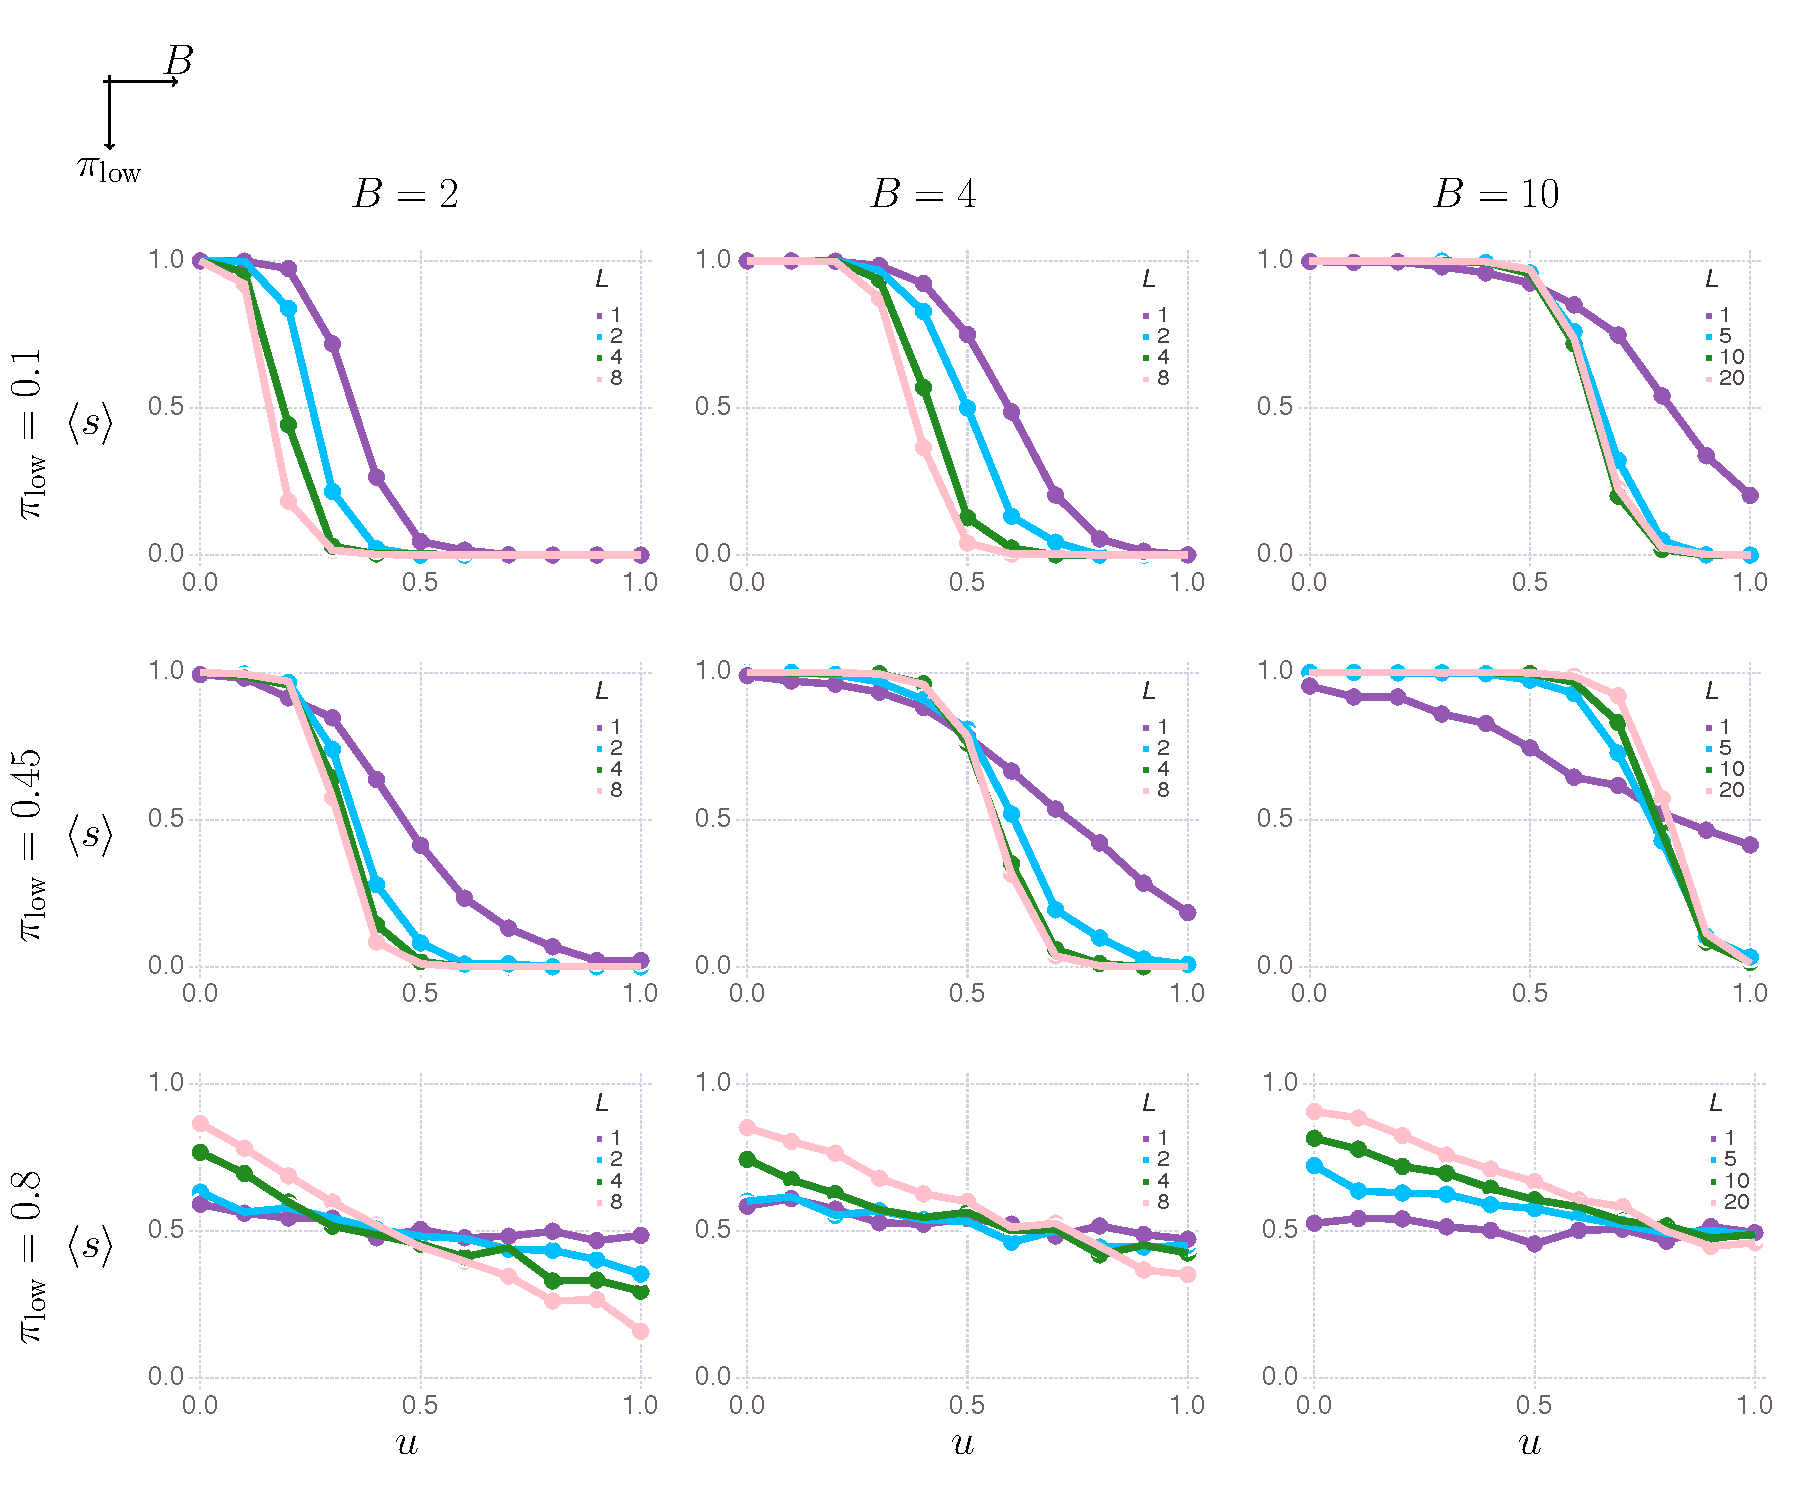
\includegraphics[width=\textwidth]{Figures/mainResultsPlots.pdf}
\end{figure}


\paragraph{Analysis 2: evolutionary uncertainty when $\meansoc \approx \meanasoc$}

\begin{figure}
  \caption{Mean payoff normalized for lifespan (y-axes, solid line with circles)
    generally track either expected all-social-learners payoff ($\meansoc$, dash-dot
    line with diamonds) or expected all-asocial payoff ($\meanasoc$, long dash
    horizontal lines) as $u$ increases (x-axes). When $\meansl$ goes from 1 to
  0 is when social learning payoffs approach individual learning payoffs due to
increased environmental variability.} 
  \label{fig:netPayoffs}
\centering
    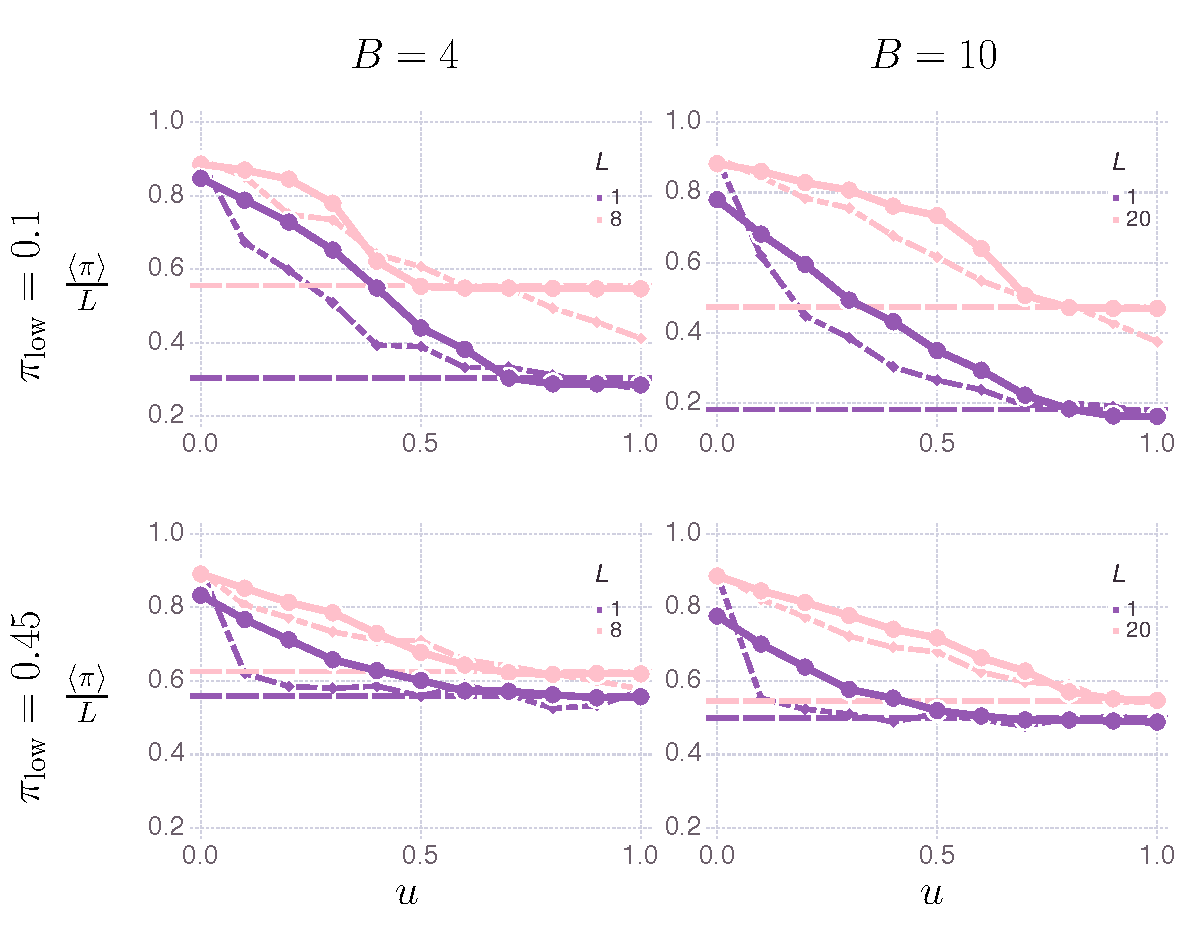
\includegraphics[width=0.75\textwidth]{Figures/meanNetPayoffs.pdf}
\end{figure}


\begin{figure}
  \caption{Average number of generations ($\meanT/L$, y-axes) for populations to fixate
  where agents either all become social or all become asocial learners. As
  $u$ increases (x-axes) models take longer to fixate due to drift, up to a point,
but then fixation accelerates as individual learning becomes more obviously 
superior. Increased $\pilow$ increases time to fixate; both $\pilow$ and $B$
shift peak time to fixation over $u$.} 
  \label{fig:steps}
\centering
    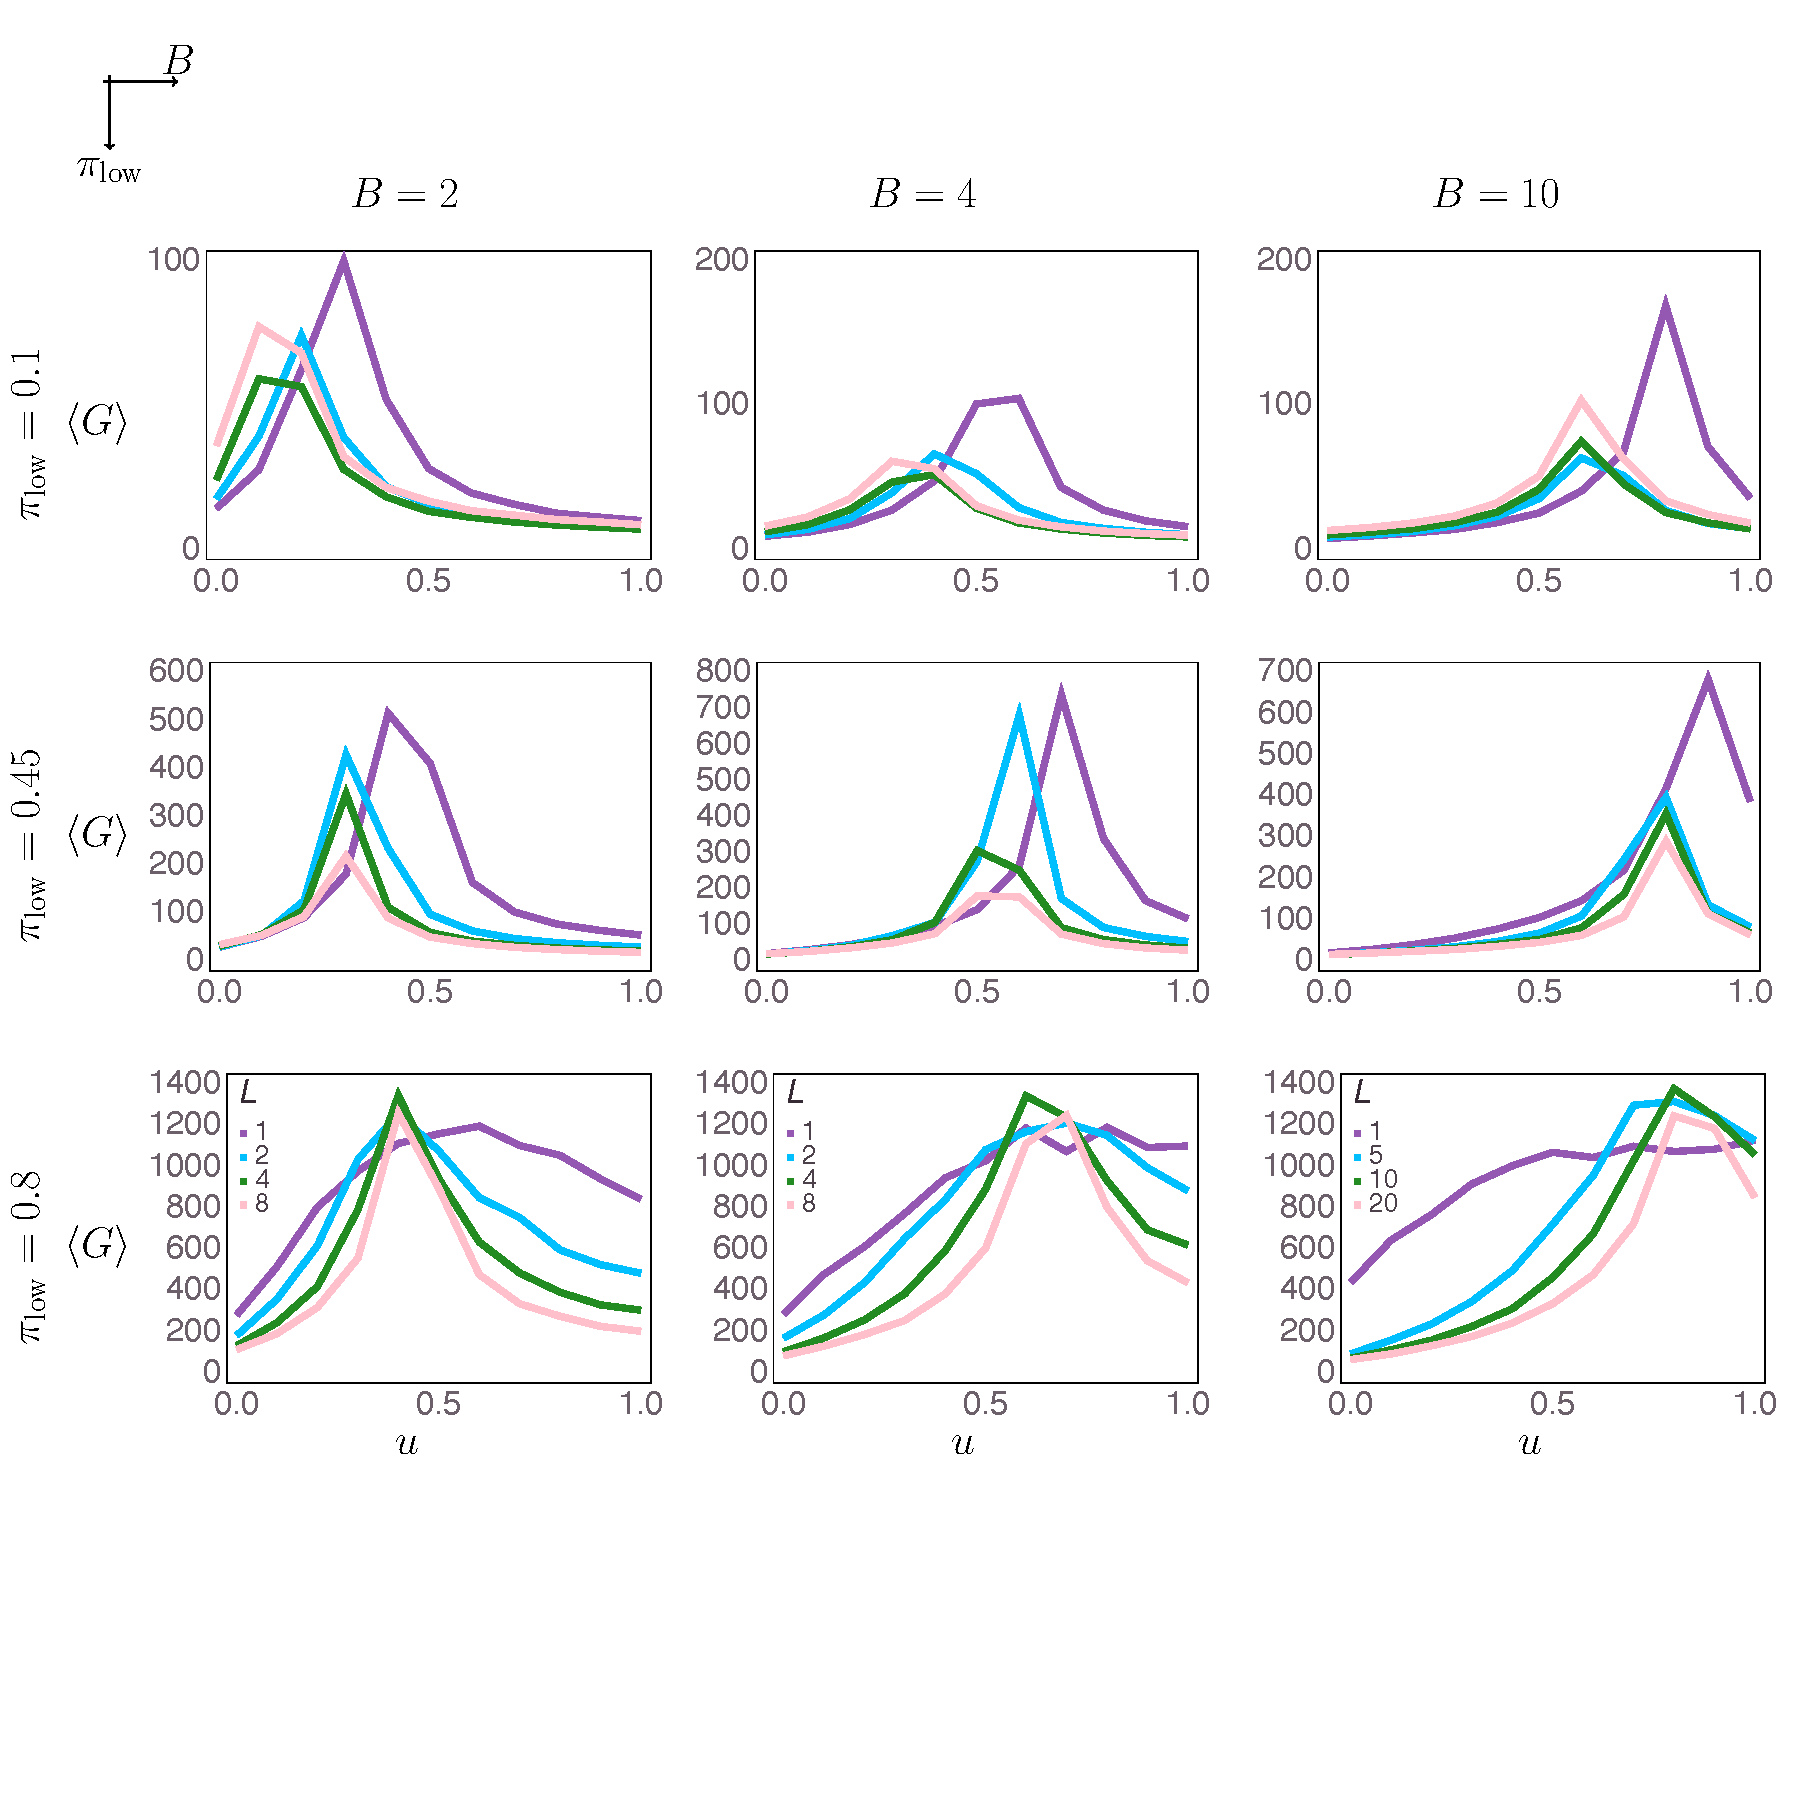
\includegraphics[width=0.75\textwidth]{Figures/stepResultsPlots.pdf}
\end{figure}

\section{Discussion}

By identifying four common uncertainty dimensions we were able to develop a model
that predicts how they might interact to foster or suppress social learning.
The model reproduced classic predictions that social learning can yield higher
payoffs than individual learning, but only up to some upper uncertainty bound.
By disambiguating and organizing various operationalizations of \emph{uncertainty},
we were able to add more detail to our theoretical understanding of which forms
of uncertainty interact in which ways to make social learning more or less
beneficial compared to asocial learning. When expected social learning payoffs
approached asocial learning payoffs the system exhibited far stronger drift; when
social or asocial learning were more obviously better the systems more consistently
evolved to the more profitable state. Note that in many cases we made modeling choices
that excluded some important mechanisms of social learning; for example we 
assumed success-biased learning, although conformity is theoretically important
as well~\cite{Muthukrishna2016a,Smaldino2018b}. Nonetheless, we believe our model
advances theoretical parsimony; and the software implementation is designed to
facilitate testing alternate modeling choices. 

\paragraph{Disc. 2: Foundation for studying social learning evolution with group
structure (PAUL, JAMIE, CRISTINA)}~\cite{Katsnelson2014}.

Our modeling approach may have applications to developing social artificial 
intelligence. Much effort has gone in to developing the cognitive machinery
to realize multi-agent reinforcement learning
systems~\cite{Sandholm1996,Ndousse2021,Gronauer2022}, with some work explicitly
incorporating cultural evolutionary approaches to social learning~\cite{Jaques2019}.
However, it seems there are a lack of methods for adapting
to environmental uncertainty, or determining when social learning is actually
advantageous under different uncertainty conditions. Our model dynamics could
be used as an evolutionary algorithm to update AI agents' social learning
strategy without knowledge of the underlying uncertainty structure.
Our model could also predict the expected benefit of social learning,
which may be inherently costly in artificial multi-agent learning systems, 
and how long the translated evolutionary algorithm may take to converge.



\bibliographystyle{apacite}
\bibliography{/Users/mt/workspace/Writing/library.bib}

\end{document}
